% Chapter 1: molecular biology primer and linear models.
% Requires: amsmath, amssymb, bm, graphicx, booktabs, multirow, subcaption, algorithm, algpseudocode,
% tikz (arrows.meta, positioning, calc, decorations.pathreplacing, decorations.pathmorphing, fit), natbib.
% Computed figures are produced by scripts/make_figures.py; figures/slides/ holds figures taken from the lecture slides.

\providecommand{\R}{\mathbb{R}}
\providecommand{\E}{\mathbb{E}}
\providecommand{\Normal}{\mathcal{N}}
\providecommand{\argmax}{\operatorname*{arg\,max}}
\providecommand{\argmin}{\operatorname*{arg\,min}}
\providecommand{\vy}{\mathbf{y}}
\providecommand{\vx}{\mathbf{x}}
\providecommand{\mX}{\mathbf{X}}
\providecommand{\mI}{\mathbf{I}}
\providecommand{\vb}{\boldsymbol{\beta}}
\providecommand{\veps}{\boldsymbol{\epsilon}}
\providecommand{\vp}{\mathbf{p}}
\providecommand{\vg}{\mathbf{g}}
\providecommand{\ind}{\mathbf{1}}

\chapter{Molecular biology basics and linear models}
\label{ch:regression}

This chapter has two goals. The first is to introduce enough molecular biology to understand where functional genomic data comes from: DNA, RNA, genes, and how sequencing turns the molecular state of a sample into numbers. The second is to develop the linear models that will serve as baselines, and often as building blocks, for the rest of the book: linear regression, its regularized variants ridge and lasso, and logistic regression for binary and multiclass outcomes. A running example connects the two halves, predicting how sensitive a cancer cell line is to a drug from its gene expression.

%======================================================================
\section{Why sequencing?}
%======================================================================

The cost of DNA sequencing has fallen faster than Moore's law for much of the last two decades (Figure~\ref{fig:seqcost}). The Human Genome Project cost roughly \$3 billion. By the mid-2010s Illumina instruments had brought the cost of a human genome to around \$1000, and in 2022 Ultima Genomics announced a ``\$100 genome'' while Illumina's NovaSeq X targeted around \$200. Alongside the incumbent short-read technology, companies such as Oxford Nanopore compete on read length. For a computational researcher this means data is abundant: the bottleneck has moved from generating measurements to interpreting them.

\begin{figure}[t]
  \centering
  \includegraphics[width=0.75\linewidth]{slides/sequencing_cost.pdf}
  \caption{Cost per megabase of DNA sequence over time. The steep drop around 2008 corresponds to the arrival of second-generation (short-read) sequencing. The first human genome (Human Genome Project) cost roughly \$3 billion; later milestones are the ``\$1000 genome'' and the ``\$100 genome''. Data from the NHGRI Genome Sequencing Program~\citep{wetterstrand} and Ultima Genomics announcements.}
  \label{fig:seqcost}
\end{figure}

\subsection{DNA sequencing}

Sequencing was first used to read genomes, either of different species or of different individuals of the same species (usually humans). Comparing the genomes of species is the domain of \emph{comparative genomics}. Regions that are conserved across species are likely to be functionally important, and differences between, for example, human and chimpanzee genomes inform the study of evolution. Comparing the genomes of individuals underpins \emph{population genetics}, which studies how genetic variation in a population arises and changes through bottlenecks, migration and selection, and \emph{statistical genetics}, which relates genetic variation to traits.

\subsection{Statistical genetics}

Statistical genetics asks how genotype (an individual's genetic make-up) is associated with phenotype (a trait), and ideally which of those associations are causal. The trait might be quantitative, like height, or a disease. For example, people carry different versions (\emph{alleles}) of the gene \textit{APOE}, and these alleles confer different risks of Alzheimer's disease. More generally we want to know which genetic differences, and which genes, contribute to a phenotype. That knowledge can guide the design of drugs that intervene on the relevant genes, or the breeding and engineering of crops that are more resilient to climate change.

One motivation for genome-wide association studies (GWAS) comes from retrospective analyses of drug development. Drug targets that are supported by human genetic evidence are at least twice as likely to progress from clinical trials to approval as targets without such support (Figure~\ref{fig:genetic_support}). The genetic evidence can come from Mendelian disease genes, catalogued in Online Mendelian Inheritance in Man (OMIM), or from GWAS, where linking an associated variant to a gene requires additional information such as linkage disequilibrium, expression quantitative trait loci (eQTLs) and enhancer-gene maps.

\begin{figure}[t]
  \centering
  \includegraphics[width=0.75\linewidth]{slides/genetic_support_odds_ratio.png}
  \caption{Odds ratio of a drug target-indication pair progressing through clinical development when the target gene has genetic support for the indication, by source of genetic evidence. OMIM, Online Mendelian Inheritance in Man; GWASdb, a database of genome-wide association study results. Reproduced from \citet{nelson2015}; see \citet{king2019} for revised estimates.}
  \label{fig:genetic_support}
\end{figure}

\subsection{Functional genomics}

Functional genomics uses sequencing for a different task, measuring the state of cells or tissue samples. ``Functional'' refers to using these measurements to understand how cells and genes function, that is, how they carry out the processes they need to survive and respond to their environment. The typical workflow is shown in Figure~\ref{fig:fg_loop}. We take a sample of cells, from an experiment or a patient, and use biochemistry to convert the quantity we want to measure into DNA molecules. We then sequence that DNA. The computational task is to infer the original state of the cells from the sequencing reads.

\begin{figure}[t]
  \centering
  \begin{tikzpicture}[>=Stealth, node distance=3.2cm, every node/.style={font=\small}]
    \node (cells) {
      \tikz{\foreach \x/\y in {0/0,0.35/0.2,0.7/-0.05,0.15/-0.4,0.55/-0.35,0.9/0.3}
              \draw[fill=gray!15] (\x,\y) circle (0.12);}
    };
    \node[below=0.05cm of cells] {cells};
    \node[right=of cells, align=center] (dna) {DNA\\molecules};
    \node[right=of dna] (reads) {reads};
    \draw[->, thick] (cells) -- node[above, align=center] {biochemistry} (dna);
    \draw[->, thick] (dna) -- node[above] {sequencing} (reads);
    \draw[->, thick] (reads.south) to[out=-110, in=-70] node[below] {computational inference} (cells.south east);
  \end{tikzpicture}
  \caption{The functional genomics workflow. A molecular quantity of interest in a sample of cells is converted to DNA, the DNA is sequenced, and computational methods infer the state of the cells from the reads.}
  \label{fig:fg_loop}
\end{figure}

%======================================================================
\section{A molecular biology primer}
%======================================================================

\subsection{The central dogma}

The central dogma of molecular biology describes the flow of information in a cell. DNA, the long-term information store, is \emph{transcribed} into RNA, which mostly acts as an intermediate ``messenger''. RNA is then \emph{translated} into protein, the worker molecules of the cell, such as enzymes and structural proteins. The three molecules differ in abundance (Table~\ref{tab:central_dogma}). A human cell typically has two copies of its DNA, one inherited from each parent, while the number of RNA and protein copies of a given gene ranges from zero to tens or thousands.

\begin{table}[t]
  \centering
  \caption{The central dogma and typical copy numbers per cell for one gene. RNA and protein counts vary widely between genes and cell types; the values are orders of magnitude.}
  \label{tab:central_dogma}
  \begin{tabular}{lll}
    \toprule
    Molecule & Role & Copies per cell \\
    \midrule
    DNA & long-term information store & 2 \\
    \quad $\downarrow$ transcription & & \\
    RNA & intermediate (messenger) & 0--30 \\
    \quad $\downarrow$ translation & & \\
    Protein & ``worker'' molecules, e.g.\ enzymes, structural & 0--$10^4$ \\
    \bottomrule
  \end{tabular}
\end{table}

\subsection{Genomes, chromosomes and genes}

The genome is divided into chromosomes, each a long DNA molecule; a human chromosome is of the order of $10^8$ base pairs long. Genes are the segments of a chromosome that are transcribed, and the stretches between them are \emph{intergenic} regions (Figure~\ref{fig:cell}). In a eukaryotic cell the chromosomes are held in the nucleus. When a gene is expressed, it is transcribed into RNA molecules in the nucleus, typically of the order of 1000 nucleotides (nt) long. The RNA is exported to the cytoplasm, where it is translated into protein. Some proteins return to the nucleus and regulate the transcription of other genes, which closes a feedback loop that we will meet again when we study gene regulation.

\begin{figure}[t]
  \centering
  \begin{tikzpicture}[>=Stealth, every node/.style={font=\small}, scale=0.95]
    % chromosome with genes
    \draw[thick] (0,0) -- (11,0);
    \draw (0,-0.12) -- (0,0.12); \draw (11,-0.12) -- (11,0.12);
    \foreach \x in {1.2, 2.8, 5.0, 7.0, 9.3}
      \draw[fill=blue!20] (\x,-0.15) rectangle (\x+0.6,0.15);
    \node[left] at (0,0) {chromosome};
    \node[above] at (6.1,0.5) {genes};
    \draw[->] (5.9,0.55) -- (5.4,0.2);
    \draw[->] (6.3,0.55) -- (7.1,0.2);
    \draw[decorate, decoration={brace, mirror, amplitude=4pt}] (5.65,-0.25) -- (6.95,-0.25)
      node[midway, below=4pt] {intergenic};
    \node[right] at (11,0) {$\sim 10^8$ bp};
    % cell
    \begin{scope}[yshift=-3.6cm]
      \draw[thick] (3.2,0) ellipse (3.6cm and 2.3cm);
      \draw[thick, fill=gray!8] (1.6,-0.2) circle (1.3cm);
      \node (nuc) at (3.5,-1.45) {nucleus};
      \draw (nuc.west) -- (2.66,-0.95);
      \node at (4.4,1.75) {cytoplasm};
      \node at (6.4,-1.9) {cell};
      \draw[decorate, decoration={snake, amplitude=1.5mm, segment length=7mm}] (0.6,-0.7) -- (2.4,-0.8);
      \draw[fill=blue!20] (1.2,-0.83) rectangle (1.6,-0.57);
      \node[below] at (1.4,-0.85) {\footnotesize gene};
      \draw[->] (1.4,-0.5) -- (1.4,0.0) node[midway, right] {\footnotesize transcription};
      \draw[decorate, decoration={snake, amplitude=0.6mm, segment length=2mm}, red!70!black] (1.1,0.2) -- (1.8,0.2);
      \draw[decorate, decoration={snake, amplitude=0.6mm, segment length=2mm}, red!70!black] (1.1,0.45) -- (1.8,0.45);
      \node[above] at (1.45,0.5) {\footnotesize RNA};
      \draw[->] (2.5,0.5) -- (3.6,0.9) node[midway, above, sloped] {\footnotesize export};
      \draw[decorate, decoration={snake, amplitude=0.6mm, segment length=2mm}, red!70!black] (3.7,0.9) -- (4.5,0.9);
      \draw[->] (4.6,0.8) to[out=-30, in=60] node[right] {\footnotesize translation} (5.0,-0.4);
      \draw[fill=orange!40] (5.0,-0.65) circle (0.22);
      \node[below] at (5.0,-0.9) {\footnotesize protein};
      \draw[->, dashed, green!50!black] (4.75,-0.65) -- (2.95,-0.4) node[midway, below] {\footnotesize regulation};
    \end{scope}
    % RNA and reads
    \begin{scope}[xshift=8.6cm, yshift=-2.2cm]
      \draw[red!70!black, decorate, decoration={snake, amplitude=0.6mm, segment length=2mm}] (0,0) -- (2.2,0);
      \draw[<->] (0,-0.3) -- (2.2,-0.3) node[midway, below] {\footnotesize RNA, $\sim$1000 nt};
      \draw[->] (1.1,-0.9) -- (1.1,-1.7) node[midway, right] {\footnotesize sequence};
      \foreach \x/\y in {0/-2.0, 0.6/-2.15, 1.3/-2.0, 0.3/-2.3, 1.0/-2.45}
        \draw[thick] (\x,\y) -- (\x+0.7,\y);
      \node[below, align=center] at (1.1,-2.5) {\footnotesize reads (substrings),\\ \footnotesize $\sim$100--150 nt};
    \end{scope}
  \end{tikzpicture}
  \caption{Genes are segments of chromosomes separated by intergenic regions (top). In the nucleus a gene is transcribed into RNA, which is exported to the cytoplasm and translated into protein; some proteins feed back to regulate transcription (bottom). Sequencing RNA produces reads that are short substrings of the RNA molecules (right).}
  \label{fig:cell}
\end{figure}

\subsection{DNA}

DNA is a double-stranded polymer of four nucleotides, A, T, G and C. The two strands are complementary: A pairs with T and C pairs with G (Figure~\ref{fig:dna}). Each strand has a direction, written from its $5'$ end to its $3'$ end, and the two strands run in opposite directions. By convention we call one strand the forward ($+$) strand and the other the reverse ($-$) strand, so that a sequence read from the reverse strand is the reverse complement of the forward sequence. Separating the strands is the first step both in duplicating DNA, during mitosis (asexual cell division) and meiosis (the cell division that produces gametes for sexual reproduction), and in transcription.

\begin{figure}[t]
  \centering
  \begin{tikzpicture}[>=Stealth, every node/.style={font=\small}]
    \draw[thick] (0,0) -- (0,-3.2); \draw[thick] (1.6,0) -- (1.6,-3.2);
    \node[above] at (0,0) {$5'$}; \node[below] at (0,-3.2) {$3'$};
    \node[above] at (1.6,0) {$3'$}; \node[below] at (1.6,-3.2) {$5'$};
    \foreach \a/\b [count=\i] in {A/T, T/A, T/A, C/G, G/C} {
      \draw (0,-0.55*\i) -- (0.25,-0.55*\i); \draw (1.35,-0.55*\i) -- (1.6,-0.55*\i);
      \node at (0.45,-0.55*\i) {\a}; \node at (1.15,-0.55*\i) {\b};
      \draw[dotted] (0.62,-0.55*\i) -- (0.98,-0.55*\i);
    }
    \draw[->] (-0.5,-0.4) -- (-0.5,-2.6) node[midway, left] {forward ($+$)};
    \draw[->] (2.1,-2.6) -- (2.1,-0.4) node[midway, right] {reverse ($-$)};
    % fate of separated strands
    \node[align=center] (sep) at (6.2,-1.6) {separate\\strands};
    \node (dup) at (8.4,-0.6) {duplication};
    \node (tx) at (8.4,-2.6) {transcription};
    \node[align=left] (mit) at (10.8,-0.1) {mitosis (asexual)};
    \node[align=left] (mei) at (10.8,-1.1) {meiosis (sexual)};
    \draw[->] (sep) -- (dup); \draw[->] (sep) -- (tx);
    \draw[->] (dup) -- (mit.west); \draw[->] (dup) -- (mei.west);
  \end{tikzpicture}
  \caption{DNA is a double-stranded polymer. The strands are complementary (A--T, C--G) and antiparallel. Strand separation is required for duplication and for transcription.}
  \label{fig:dna}
\end{figure}

\subsection{RNA and gene expression}

RNA uses the same nucleotides as DNA except that thymine (T) is replaced by uracil (U). The number of RNA copies of a gene in a cell is what we call that gene's \emph{expression}. Cells control expression in response to three kinds of question: \emph{when} (for example at different stages of development), \emph{where} (in which tissues and cell types) and \emph{why} (in response to a stimulus, for example an immune challenge). The mechanisms by which they do so are collectively called \emph{gene regulation}.

\subsection{RNA-seq}

RNA sequencing (RNA-seq) measures gene expression (Figure~\ref{fig:rnaseq}). RNA molecules are extracted from cells; they are typically of the order of 1000 nt long. The RNA is fragmented and reverse transcribed into complementary DNA (cDNA), giving fragments of around 300--400 nt. The cDNA is sequenced, producing reads of around 100--150 nt; a typical experiment yields 30--100 million reads per sample. The reads are aligned to the genome, and the number of reads overlapping each gene is counted. These counts, suitably normalized, are the gene expression measurements we will model.

\begin{figure}[t]
  \centering
  \begin{tikzpicture}[>=Stealth, node distance=0.9cm, every node/.style={font=\small, align=center}]
    \node (cells) {cells};
    \node[right=of cells] (rna) {RNA molecules\\$\sim$1000 nt};
    \node[right=2.6cm of rna] (cdna) {cDNA fragments\\$\sim$300--400 nt};
    \node[below=1.3cm of cdna] (reads) {reads, $\sim$100--150 nt\\30--100M per sample};
    \node[left=1.3cm of reads] (align) {align to\\genome};
    \node[left=of align] (count) {count reads\\per gene};
    \node[left=of count] (expr) {gene\\expression};
    \draw[->] (cells) -- node[above] {extract} (rna);
    \draw[->] (rna) -- node[above, font=\footnotesize] {fragment,} node[below, font=\footnotesize] {reverse} node[below=0.3cm, font=\footnotesize] {transcribe} (cdna);
    \draw[->] (cdna) -- node[right] {sequence} (reads);
    \draw[->] (reads) -- (align);
    \draw[->] (align) -- (count);
    \draw[->] (count) -- (expr);
    % reads piling up on a gene
    \begin{scope}[shift={($(align.south)+(-1.4,-0.9)$)}]
      \draw (0,0) -- (2.8,0);
      \draw[fill=blue!20] (0.9,-0.1) rectangle (1.9,0.1);
      \foreach \x/\y in {0.85/0.25, 1.15/0.25, 1.45/0.25, 1.0/0.4, 1.3/0.4, 1.6/0.4}
        \draw[thick] (\x,\y) -- (\x+0.35,\y);
    \end{scope}
  \end{tikzpicture}
  \caption{The RNA-seq workflow. Read counts per gene, after normalization, are used as measurements of gene expression.}
  \label{fig:rnaseq}
\end{figure}

Bulk RNA-seq is applied to a tissue sample containing many cells, so it measures the average expression across all cells in the sample. Single-cell RNA-seq (scRNA-seq) measures expression in individual cells, which reveals heterogeneity between cell types that bulk measurements average over (Figure~\ref{fig:bulk_sc}). We will return to single-cell data in later chapters.

\begin{figure}[t]
  \centering
  \includegraphics[width=0.85\linewidth]{slides/bulk_vs_singlecell.png}
  \caption{Bulk RNA-seq measures the average expression across all cells in a sample, masking differences between cell types. Single-cell RNA-seq measures each cell separately and can reveal subpopulations. Reproduced from \citet{tenx_blog}.}
  \label{fig:bulk_sc}
\end{figure}

%======================================================================
\section{Application: predicting cancer drug sensitivity}
\label{sec:drug_app}
%======================================================================

Cancer cell lines are populations of cells derived from patient tumours that can be grown in culture indefinitely (Figure~\ref{fig:culture}). Each line can be profiled with RNA-seq and other assays, and in parallel screened for its sensitivity to a panel of drugs. Several consortia have generated such data at scale, including the Cancer Cell Line Encyclopedia (CCLE)~\citep{barretina2012}, Genomics of Drug Sensitivity in Cancer (GDSC)~\citep{garnett2012} and the Cancer Therapeutics Response Portal (CTRP)~\citep{seashore2015}. The resulting data can be arranged as two matrices with a shared row index (Figure~\ref{fig:data_matrices}a). The expression matrix has one row per cell line and one column per gene. The sensitivity matrix has one row per cell line and one column per drug. Predicting the sensitivity of cell lines to one drug, say drug A, from their gene expression is a regression problem, and it is the running example of the first half of this chapter.

\begin{figure}[t]
  \centering
  \includegraphics[width=0.5\linewidth]{slides/primary_culture.png}
  \caption{Deriving a primary cancer cell culture from tumour tissue: dissociation into single cells, cultivation, and depletion of non-malignant cells. The resulting lines can be profiled (e.g.\ by RNA-seq) and screened for drug sensitivity. \textbf{[Source to be confirmed.]}}
  \label{fig:culture}
\end{figure}

\begin{figure}[t]
  \centering
  \begin{tikzpicture}[>=Stealth, every node/.style={font=\small, align=center}]
    \node at (-1.0,3.6) {(a)};
    \draw[thick] (0,0) rectangle (3.2,3.0);
    \node at (1.6,1.5) {gene expression\\from RNA-seq\\[2pt] $\mX$};
    \node[above] at (1.6,3.0) {$\sim$20{,}000 genes};
    \node[rotate=90] at (-0.35,1.5) {$\sim$1000 cell lines};
    \draw[thick] (4.0,0) rectangle (6.4,3.0);
    \draw[fill=orange!25] (4.0,0) rectangle (4.35,3.0);
    \node at (5.4,1.5) {drug\\sensitivity};
    \node[above] at (5.2,3.0) {$\sim$1000 drugs};
    \draw[<-] (4.17,-0.1) -- (4.17,-0.6) node[below] {drug A, $\vy$};
    % Oncotype DX
    \begin{scope}[xshift=8.0cm]
      \node at (-1.0,3.6) {(b)};
      \draw[thick] (0,0.4) rectangle (3.2,2.6);
      \node at (1.6,1.5) {gene expression\\$\mX$};
      \node[above] at (1.6,2.6) {$\sim$10{,}000 genes};
      \node[rotate=90] at (-0.35,1.5) {$\sim$700 patients};
      \draw[thick, fill=orange!25] (3.6,0.4) rectangle (3.95,2.6);
      \node[right] at (4.0,1.5) {$\vy$};
      \node[below, align=center] at (3.8,0.3) {recurrence or\\metastasis\\within 10 years};
    \end{scope}
  \end{tikzpicture}
  \caption{Data matrices for the two applications in this chapter. (a) Cancer cell line drug screens: an expression matrix $\mX$ (cell lines $\times$ genes) and a sensitivity matrix (cell lines $\times$ drugs). Predicting one column $\vy$ of the sensitivity matrix from $\mX$ is a regression problem. (b) Predicting breast cancer recurrence from tumour gene expression (Section~\ref{sec:classification}) is a binary classification problem.}
  \label{fig:data_matrices}
\end{figure}

Sensitivity is summarized from a dose-response experiment for each drug-cell line pair (Figure~\ref{fig:dose_response}). The cell line is grown at a series of drug concentrations and its growth is measured relative to untreated cells. Two common summaries are the IC$_{50}$, the concentration at which growth is reduced by half, and the \emph{activity area}, the area between the dose-response curve and 100\% growth. A larger activity area means a more sensitive cell line. The CCLE study, for example, screened 24 drugs across 479 cell lines spanning many tumour types (Figure~\ref{fig:ccle_types})~\citep{barretina2012}.

\begin{figure}[t]
  \centering
  \begin{subfigure}[b]{0.48\linewidth}
    \includegraphics[width=\linewidth]{slides/ccle_tumour_types.png}
    \caption{}
    \label{fig:ccle_types}
  \end{subfigure}\hfill
  \begin{subfigure}[b]{0.48\linewidth}
    \includegraphics[width=\linewidth]{dose_response.pdf}
    \caption{}
    \label{fig:dose_response}
  \end{subfigure}
  \caption{(a) Number of cell lines by tumour type in the CCLE drug screen, reproduced from \citet{barretina2012}. (b) Schematic dose-response curve for a single drug-cell line pair. The IC$_{50}$ is the concentration at which growth falls to 50\% of untreated; the activity area (shaded) is the area between the curve and 100\% growth.}
\end{figure}

%======================================================================
\section{Linear regression}
\label{sec:linreg}
%======================================================================

Linear regression models a continuous \emph{response} (also called the dependent variable or output), such as drug sensitivity, as a linear function of one or more \emph{inputs} (features, independent variables, covariates), such as gene expression levels (Figure~\ref{fig:linreg}).

\begin{figure}[t]
  \centering
  \includegraphics[width=0.6\linewidth]{linreg_scatter.pdf}
  \caption{Linear regression with one covariate. Each point is a sample; the line is the least-squares fit.}
  \label{fig:linreg}
\end{figure}

\subsection{The model}

Let $N$ be the number of samples (cell lines) and $P$ the number of features (genes). We index samples by $i\in\{1,\dots,N\}$ and features by $j\in\{1,\dots,P\}$. Let $y_i\in\R$ be the response of sample $i$, $X_{ij}\in\R$ the expression of gene $j$ in sample $i$, $\beta_j\in\R$ the coefficient of gene $j$, and $\epsilon_i\in\R$ a noise term. The linear regression model is
\begin{equation}
  y_i = \sum_{j=1}^P X_{ij}\beta_j + \epsilon_i + \mu ,
  \label{eq:linreg_scalar}
\end{equation}
where $\mu$ is an intercept. A coefficient $\beta_j=0$ means gene $j$ has no effect on the response; $\beta_j<0$ means higher expression of gene $j$ is associated with lower sensitivity. We will usually assume $\vy$ has been centered (mean zero), so that $\mu=0$, or equivalently absorb the intercept into $\vb$ by appending a column of ones to the features. The responses and features are observed; the coefficients are the unknowns we want to estimate; the noise is a nuisance.

In vector notation, let $\vx_i\in\R^{P}$ be the features of sample $i$ (as a column vector) and $\vb\in\R^P$ the coefficient vector. Then $y_i = \vx_i^\top\vb + \epsilon_i$, where $\vx_i^\top$ is $1\times P$ and $\vb$ is $P\times 1$, so their inner product is a scalar. Stacking samples, let $\vy\in\R^N$, let $\mX\in\R^{N\times P}$ be the matrix whose $i$-th row is $\vx_i^\top$, and let $\veps\in\R^N$. The model is
\begin{equation}
  \underbrace{\vy}_{N\times 1} = \underbrace{\mX}_{N\times P}\;\underbrace{\vb}_{P\times 1} + \underbrace{\veps}_{N\times 1}, \qquad \epsilon_i \overset{\text{iid}}{\sim} \Normal(0,\sigma^2),
  \label{eq:linreg}
\end{equation}
where $\sigma^2$ is the noise variance and ``iid'' means independent and identically distributed. We write $\mX_{:j}\in\R^N$ for the $j$-th column of $\mX$, the expression of gene $j$ across samples.

\subsection{Likelihood}

The likelihood is the probability of the observed data as a function of the parameters, $L(\vb)=p(\mathcal{D}\mid\vb)=p(\vy\mid\mX,\vb)$, where $\mathcal{D}$ denotes the data. Since $\epsilon_i=y_i-\vx_i^\top\vb$ is Gaussian, the likelihood of one sample is
\begin{equation}
  p(y_i\mid\vx_i,\vb) = \frac{1}{\sqrt{2\pi\sigma^2}}\exp\left(-\frac{1}{2\sigma^2}(y_i-\vx_i^\top\vb)^2\right).
\end{equation}
Because the noise terms are independent, the likelihood of all samples is the product
\begin{equation}
  p(\vy\mid\mX,\vb) = \prod_{i=1}^N p(y_i\mid\vx_i,\vb) = \frac{1}{(2\pi\sigma^2)^{N/2}}\exp\left(-\frac{1}{2\sigma^2}\sum_{i=1}^N(y_i-\vx_i^\top\vb)^2\right),
\end{equation}
and the log likelihood is
\begin{equation}
  \log L(\vb) = -\frac{N}{2}\log 2\pi\sigma^2 - \frac{1}{2\sigma^2}\sum_{i=1}^N\left(y_i-\vx_i^\top\vb\right)^2 .
  \label{eq:loglik}
\end{equation}
The first term does not depend on $\vb$, so maximizing the log likelihood over $\vb$ is equivalent to minimizing the sum of squared errors $\sum_i(y_i-\vx_i^\top\vb)^2$.

\subsection{Finding the optimal parameters}

The log likelihood~\eqref{eq:loglik} is a concave quadratic in $\vb$, so its maximum is where the gradient is zero,
\begin{equation}
  \nabla_{\vb}\log L = \frac{1}{\sigma^2}\sum_{i=1}^N \vx_i\left(y_i-\vx_i^\top\vb\right) = 0
  \quad\Rightarrow\quad
  \sum_{i=1}^N \vx_i\vx_i^\top\vb = \sum_{i=1}^N\vx_i y_i .
\end{equation}
In matrix notation this is $\mX^\top\mX\vb = \mX^\top\vy$, with dimensions $[P\times N][N\times P][P\times 1]=[P\times N][N\times 1]$. Solving gives the maximum likelihood estimate (MLE), also known as the ordinary least squares (OLS) estimate,
\begin{equation}
  \hat\vb = (\mX^\top\mX)^{-1}\mX^\top\vy .
  \label{eq:ols}
\end{equation}
In practice we do not form the inverse explicitly. Equation~\eqref{eq:ols} has the form $\mathbf{A}\vb=\mathbf{c}$ with $\mathbf{A}=\mX^\top\mX$ and $\mathbf{c}=\mX^\top\vy$, so we call a linear solver, $\hat\vb=\texttt{solve}(\mX^\top\mX,\mX^\top\vy)$, which is faster and numerically more stable.

\subsection{Special case: independent covariates}

Suppose $\vy$ and each column $\mX_{:j}$ have been standardized to mean zero and variance one, and that the features are uncorrelated, $\operatorname{corr}(\mX_{:j},\mX_{:k})=0$ for $j\neq k$. Then $\mX^\top\mX=N\mI$, where $\mI$ is the $P\times P$ identity, and
\begin{equation}
  \hat\vb = (N\mI)^{-1}\mX^\top\vy = \frac{1}{N}\mX^\top\vy, \qquad \hat\beta_j = \frac{1}{N}\mX_{:j}^\top\vy = \operatorname{corr}(\mX_{:j},\vy).
\end{equation}
When features are uncorrelated, the regression coefficient of gene $j$ is the correlation between its expression and the response, and each gene can be considered separately. When features are correlated, as genes usually are, the coefficients must be estimated jointly.

\subsection{\texorpdfstring{Small $N$, large $P$}{Small N, large P} and colinearity}

Genomic data sets often have more features than samples: thousands of genes but hundreds of cell lines. Since $\operatorname{rank}(\mX^\top\mX)\leq\min(N,P)$, when $N<P$ the $P\times P$ matrix $\mX^\top\mX$ is not invertible and~\eqref{eq:ols} has no unique solution. The columns of $\mX$ are then linearly dependent, a situation called \emph{colinearity}: some combination of features can be changed without changing the predictions, and the likelihood is flat along that direction.

Even when $N>P$, strongly correlated features make the problem \emph{poorly conditioned}. The condition number of $\mX^\top\mX$ is the ratio of its largest to smallest eigenvalue, $\kappa=\nu_{\max}/\nu_{\min}$. A large condition number means $\mX^\top\mX$ is close to non-invertible, and small changes to the data produce large changes in $\hat\vb$. Figure~\ref{fig:colinearity} (left) shows the sum of squares for two features with correlation $0.98$. The contours are elongated along the direction $\beta_1+\beta_2=\text{const}$: if $\vx_1\approx\vx_2$, increasing $\beta_1$ and decreasing $\beta_2$ by the same amount leaves the fit nearly unchanged, so all points along this ridge are almost equally good. Adding a penalty on the size of $\vb$ (right) makes the minimum well defined. The next section motivates such penalties.

\begin{figure}[t]
  \centering
  \includegraphics[width=0.85\linewidth]{colinearity_contours.pdf}
  \caption{Contours of the sum of squares $\sum_i(y_i-\vx_i^\top\vb)^2$ for two features with correlation $0.98$ (left) and of the ridge objective, which adds $\lambda\|\vb\|_2^2$ (right). The least-squares minimum lies in a long, flat valley and is unstable; the ridge minimum is well defined. Red points mark the minimizers.}
  \label{fig:colinearity}
\end{figure}

%======================================================================
\section{Priors, Bayes' rule and ridge regression}
\label{sec:ridge}
%======================================================================

\subsection{Bayes' rule}

For parameters $\theta$ and data $\mathcal{D}$, Bayes' rule is
\begin{equation}
  \underbrace{p(\theta\mid\mathcal{D})}_{\text{posterior}} = \frac{\overbrace{p(\mathcal{D}\mid\theta)}^{\text{likelihood}}\;\overbrace{p(\theta)}^{\text{prior}}}{\underbrace{p(\mathcal{D})}_{\text{evidence}}} ,
\end{equation}
where the evidence or \emph{marginal likelihood} $p(\mathcal{D})=\int p(\mathcal{D}\mid\theta)p(\theta)\,d\theta$ does not depend on $\theta$. For linear regression, $\mathcal{D}=\vy$ (we condition on $\mX$ throughout) and $\theta=\vb$.

A natural prior expresses the belief that most coefficients are small: each coefficient is drawn independently from a Gaussian with mean zero and variance $\sigma_\beta^2$,
\begin{equation}
  \beta_j\overset{\text{iid}}{\sim}\Normal(0,\sigma_\beta^2), \qquad p(\beta_j)=\Normal(\beta_j\mid 0,\sigma^2_\beta)=\frac{1}{\sqrt{2\pi\sigma_\beta^2}}\exp\left(-\frac{\beta_j^2}{2\sigma_\beta^2}\right).
\end{equation}
Figure~\ref{fig:prior_post} shows the prior, likelihood and posterior for a single coefficient. The posterior combines the two sources of information and is more concentrated than either.

\begin{figure}[t]
  \centering
  \includegraphics[width=0.6\linewidth]{prior_likelihood_posterior.pdf}
  \caption{Prior, likelihood (normalized to integrate to one) and posterior for a single regression coefficient with $N=5$ samples. The posterior mode (MAP) is shrunk from the maximum likelihood estimate (MLE) toward the prior mean of zero.}
  \label{fig:prior_post}
\end{figure}

\subsection{Maximum a posteriori estimation is L2 regularization}

Taking logs of Bayes' rule,
\begin{align}
  \log p(\vb\mid\vy) &= \log p(\vy\mid\mX,\vb) + \log p(\vb) - \log p(\vy) \nonumber\\
  &= -\frac{1}{2\sigma^2}\sum_{i=1}^N\left(y_i-\vx_i^\top\vb\right)^2 - \frac{1}{2\sigma_\beta^2}\sum_{j=1}^P\beta_j^2 + \text{const},
  \label{eq:logpost}
\end{align}
where the constant collects $\log p(\vy)$ and the normalizing terms $-\frac{N}{2}\log 2\pi\sigma^2-\frac{P}{2}\log 2\pi\sigma_\beta^2$, none of which depend on $\vb$. The maximum a posteriori (MAP) estimate maximizes~\eqref{eq:logpost}. Using $\nabla_{\vb}(\vb^\top\mathbf{A}\vb)=2\mathbf{A}\vb$ for symmetric $\mathbf{A}$, the gradient is
\begin{equation}
  \nabla_{\vb}\log p(\vb\mid\vy) = \frac{1}{\sigma^2}\sum_i\vx_i\left(y_i-\vx_i^\top\vb\right) - \frac{1}{\sigma_\beta^2}\vb = 0 .
\end{equation}
Rearranging, $\frac{1}{\sigma^2}\mX^\top\vy = \left(\frac{1}{\sigma^2}\mX^\top\mX + \frac{1}{\sigma_\beta^2}\mI\right)\vb$, and multiplying through by $\sigma^2$,
\begin{equation}
  \hat\vb_{\text{MAP}} = \left(\mX^\top\mX + \lambda\mI\right)^{-1}\mX^\top\vy, \qquad \lambda = \frac{\sigma^2}{\sigma^2_\beta}.
  \label{eq:ridge}
\end{equation}
This is the \emph{ridge regression} estimator~\citep{hoerl1970}. Equivalently, it minimizes the penalized loss
\begin{equation}
  \frac{1}{2}\sum_{i=1}^N\left(y_i-\vx_i^\top\vb\right)^2 + \frac{\lambda}{2}\|\vb\|_2^2 ,
\end{equation}
where $\|\vb\|_2^2=\sum_j\beta_j^2$. The added term is called \emph{L2 regularization}: it penalizes large coefficients and shrinks the estimate toward zero. Because $\lambda>0$ makes $\mX^\top\mX+\lambda\mI$ invertible for any $\mX$, ridge regression has a unique solution even when $N<P$. The regularization strength $\lambda$ is the ratio of noise variance to prior variance: a broad prior (large $\sigma_\beta^2$) or low noise means weak regularization. Only the ratio matters for $\hat\vb_{\text{MAP}}$. Scaling $\sigma^2$ and $\sigma_\beta^2$ together changes the curvature of the posterior, and therefore our uncertainty, but not its mode. Since the penalty treats all coefficients alike, features should be put on a common scale, usually by standardizing each column of $\mX$, before fitting.

Because the prior and likelihood are both Gaussian in $\vb$, the posterior is Gaussian as well, with mean $\hat\vb_{\text{MAP}}$ and covariance $\sigma^2(\mX^\top\mX+\lambda\mI)^{-1}$. For Gaussian posteriors the MAP and posterior mean coincide.

\subsection{\texorpdfstring{Choosing $\lambda$}{Choosing lambda}}

There are two common options for choosing the regularization strength.
\begin{enumerate}
  \item \emph{Cross-validation}: choose the $\lambda$ that gives the best predictions on held-out data (Section~\ref{sec:model_selection}).
  \item \emph{Empirical Bayes}, or maximum marginal likelihood: choose $\sigma^2$ and $\sigma^2_\beta$ to maximize the evidence $p(\vy\mid\mX,\sigma^2,\sigma_\beta^2)$. Integrating out $\vb$ gives $\vy\mid\mX\sim\Normal\left(\mathbf{0},\,\sigma_\beta^2\mX\mX^\top+\sigma^2\mI_N\right)$, which can be maximized numerically.
\end{enumerate}

Section 3.4.1 of \citet{esl} gives a complementary treatment of ridge regression.

%======================================================================
\section{Assessing regression performance}
\label{sec:regression_metrics}
%======================================================================

The metrics used for classification (accuracy, precision, recall, area under the ROC curve; Section~\ref{sec:classification_metrics}) do not apply directly to regression. If there is a natural threshold, one can binarize predictions and observations after fitting and then use classification metrics, but in general we want metrics designed for continuous outcomes. Let $\hat y_i=\vx_i^\top\hat\vb$ be the prediction for sample $i$.

\begin{itemize}
  \item The \emph{sum of squared errors} is $\text{SS}=\sum_i(y_i-\hat y_i)^2$. It is hard to interpret because it depends on the number of samples and on the scale of $y$.
  \item The \emph{mean squared error} $\text{MSE}=\frac{1}{N}\text{SS}$ removes the dependence on $N$, and the \emph{root mean squared error} $\text{RMSE}=\sqrt{\text{MSE}}$ is on the same scale, and in the same units, as $y$. MSE and RMSE estimate the noise variance $\sigma^2$ and standard deviation $\sigma$. This holds only if the model neither overfits, in which case they underestimate the noise, nor underfits, in which case they overestimate it.
  \item MSE and RMSE still depend on the scale of $y$, so they cannot be compared across data sets. The \emph{coefficient of determination} is
  \begin{equation}
    R^2 = 1-\frac{\text{SS}}{\text{TSS}} = 1-\frac{\text{MSE}}{s_y^2}, \qquad \text{TSS}=\sum_i(y_i-\bar y)^2,
  \end{equation}
  where $\bar y$ is the mean of $\vy$, $\text{TSS}$ is the total sum of squares and $s_y^2=\text{TSS}/N$ is the variance of the observations. For centered $\vy$, $\text{TSS}=\sum_i y_i^2$. $R^2$ is the proportion of variance explained (PVE) by the model. If $\vy$ is scaled to unit variance, $R^2=1-\text{MSE}$.
\end{itemize}

For the least-squares fit of a model with an intercept, evaluated on the training data, $R^2$ equals the squared Pearson correlation between $\vy$ and $\hat\vy$ and lies in $[0,1]$, with 0 meaning no agreement and 1 meaning perfect prediction. On held-out data the two can differ: the Pearson correlation ignores the mean and scale of the predictions, while $R^2$ does not, and held-out $R^2$ can be negative if predictions are worse than predicting the mean. Figure~\ref{fig:rmse} illustrates RMSE as the typical vertical distance of points from the fitted line.

\begin{figure}[t]
  \centering
  \begin{tikzpicture}[>=Stealth, every node/.style={font=\small}, scale=0.9]
    \draw[->] (-2.2,0) -- (3,0) node[right] {$x$};
    \draw[->] (0,-1.6) -- (0,2.4) node[above] {$y$};
    \draw[thick, blue!60!black] (-2.2,-1.32) -- (2.6,1.56);
    \foreach \x/\y in {-1.9/-0.8, -1.5/-1.4, -1.0/-0.2, -0.6/-0.75, 0.5/0.7, 0.9/0.1, 1.4/1.5, 2.0/0.85, 2.3/1.9}
      \node at (\x,\y) {$\times$};
    \draw[<->, red!70!black] (2.0,0.85) -- (2.0,1.2);
    \draw[<->, red!70!black] (-1.5,-1.4) -- (-1.5,-0.9);
    \node[right, red!70!black] at (2.1,0.6) {$\sim$RMSE};
  \end{tikzpicture}
  \caption{The RMSE is on the scale of the typical vertical deviation of observations from the fitted line.}
  \label{fig:rmse}
\end{figure}

A final summary is the statistical significance (p-value) of the Pearson or Spearman correlation between predictions and observations on held-out data. This is rarely reported in computer vision or natural language processing, but biological data are often noisy enough that $R^2$ is low and it is unclear whether we are predicting better than chance.

We sometimes describe a regression model informally as ``accurate''. For classification, accuracy has a specific meaning: the proportion of samples assigned to the correct class.

%======================================================================
\section{Model selection}
\label{sec:model_selection}
%======================================================================

\subsection{Training, validation and test sets}

To choose hyperparameters such as $\lambda$ and to assess how well a model generalizes, we split the samples into three sets (Figure~\ref{fig:splits}a). The \emph{training set} (for example 60\% of samples) is used in the likelihood or loss to fit the parameters $\vb$. The \emph{validation set} (20\%) is used to estimate the generalization error of models fit with different hyperparameters, and to pick the best. The \emph{test set} (20\%) is used once, at the end, for a final assessment of generalization. Using the test set to make modelling choices leads to optimistic estimates of performance.

\begin{figure}[t]
  \centering
  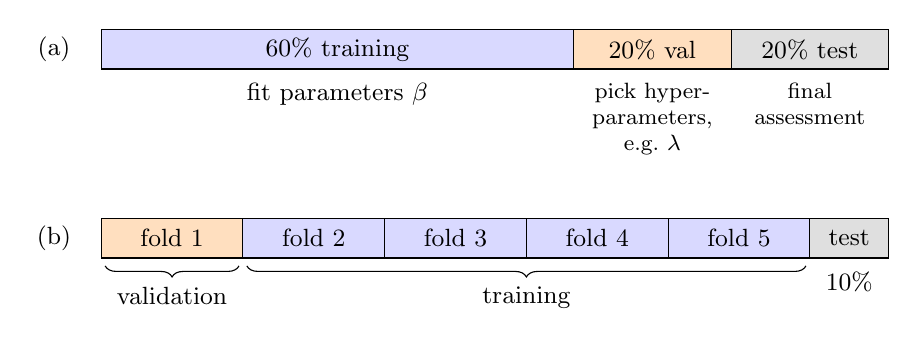
\begin{tikzpicture}[every node/.style={font=\small, align=center}]
    \node at (-0.6,0.25) {(a)};
    \draw[fill=blue!15] (0,0) rectangle (6,0.5); \node at (3,0.25) {60\% training};
    \draw[fill=orange!25] (6,0) rectangle (8,0.5); \node at (7,0.25) {20\% val};
    \draw[fill=gray!25] (8,0) rectangle (10,0.5); \node at (9,0.25) {20\% test};
    \node[below] at (3,-0.05) {fit parameters $\vb$};
    \node[below, font=\footnotesize] at (7,-0.05) {pick hyper-\\parameters,\\e.g.\ $\lambda$};
    \node[below, font=\footnotesize] at (9,-0.05) {final\\assessment};
    \begin{scope}[yshift=-2.4cm]
      \node at (-0.6,0.25) {(b)};
      \foreach \k in {0,...,4} {
        \pgfmathsetmacro{\xa}{1.8*\k}
        \pgfmathsetmacro{\xb}{1.8*(\k+1)}
        \ifnum\k=0 \def\col{orange!25}\else\def\col{blue!15}\fi
        \draw[fill=\col] (\xa,0) rectangle (\xb,0.5);
        \node at ({1.8*\k+0.9},0.25) {fold \the\numexpr\k+1\relax};
      }
      \draw[fill=gray!25] (9,0) rectangle (10,0.5); \node at (9.5,0.25) {test};
      \draw[decorate, decoration={brace, mirror, amplitude=4pt}] (0.05,-0.1) -- (1.75,-0.1) node[midway, below=4pt] {validation};
      \draw[decorate, decoration={brace, mirror, amplitude=4pt}] (1.85,-0.1) -- (8.95,-0.1) node[midway, below=4pt] {training};
      \node[below] at (9.5,-0.05) {10\%};
    \end{scope}
  \end{tikzpicture}
  \caption{(a) A training/validation/test split. (b) Five-fold cross-validation: the non-test data are split into five folds, and each fold in turn is held out for validation while the model is trained on the other four. The first round is shown.}
  \label{fig:splits}
\end{figure}

\subsection{Overfitting and underfitting}

Figure~\ref{fig:cv_curve} shows how validation error depends on $\lambda$. With $\lambda$ near zero the model is complex: it fits the noise in the training data and generalizes poorly, which is \emph{overfitting}. With large $\lambda$ the model is too simple: the coefficients are shrunk so far toward zero that the model misses real signal, which is \emph{underfitting}. The optimal $\lambda$ lies between.

\subsection{Cross-validation}

A single validation set wastes data and gives a noisy estimate of generalization error. In $K$-fold cross-validation (Figure~\ref{fig:splits}b and Algorithm~\ref{alg:cv}) the non-test data are split into $K$ folds; each fold is held out in turn while the model is trained on the rest, and the validation losses are averaged. Typical choices are $K=5$ or $K=10$. The grid of $\lambda$ values is usually spaced logarithmically.

\begin{algorithm}[t]
  \caption{$K$-fold cross-validation for choosing $\lambda$}
  \label{alg:cv}
  \begin{algorithmic}[1]
    \State Split the non-test samples into folds $F_1,\dots,F_K$
    \For{$\lambda$ in a grid, e.g.\ $\{0, 0.1, 0.5, \dots, 100, 500\}$}
      \For{$k=1,\dots,K$}
        \State Fit $\hat\vb^{(-k)}(\lambda)$ on all folds except $F_k$
        \State $\text{err}_k(\lambda)\gets$ validation loss of $\hat\vb^{(-k)}(\lambda)$ on $F_k$
      \EndFor
      \State $\text{CV}(\lambda)\gets\frac{1}{K}\sum_k\text{err}_k(\lambda)$
    \EndFor
    \State $\hat\lambda\gets\argmin_\lambda\text{CV}(\lambda)$; refit on all non-test samples with $\hat\lambda$
  \end{algorithmic}
\end{algorithm}

\begin{figure}[t]
  \centering
  \includegraphics[width=0.6\linewidth]{cv_curve.pdf}
  \caption{Five-fold cross-validation estimate of mean squared error for ridge regression on simulated data ($N=100$, $P=60$), as a function of $\lambda$. The band shows $\pm$ one standard error across folds. Small $\lambda$ overfits and large $\lambda$ underfits.}
  \label{fig:cv_curve}
\end{figure}

\subsection{The bias-variance trade-off}

Let $\vb_0$ denote the true coefficients and $\hat\vb$ an estimate computed from a random training set. For a new input $\vx$, the expected squared error of the prediction $\vx^\top\hat\vb$ for a new response $y=\vx^\top\vb_0+\epsilon$ decomposes as
\begin{equation}
  \E\left[(y-\vx^\top\hat\vb)^2\right] = \underbrace{\left(\E[\vx^\top\hat\vb]-\vx^\top\vb_0\right)^2}_{\text{bias}^2} + \underbrace{\E\left[\left(\vx^\top\hat\vb-\E[\vx^\top\hat\vb]\right)^2\right]}_{\text{variance}} + \underbrace{\sigma^2}_{\text{noise}},
\end{equation}
where the expectations are over training sets and the new noise $\epsilon$. Averaging over new inputs $\vx$ gives the generalization error. The noise term is intrinsic and cannot be reduced. Regularization trades the other two terms against each other (Figure~\ref{fig:bias_var}): increasing $\lambda$ increases bias, because estimates are shrunk away from $\vb_0$, but decreases variance, because estimates depend less on the particular training set. The optimal $\lambda$ minimizes their sum. Section 2.9 of \citet{esl} covers this in more depth.

\begin{figure}[t]
  \centering
  \includegraphics[width=0.6\linewidth]{bias_variance.pdf}
  \caption{Bias-variance decomposition of the expected prediction error of ridge regression for a fixed simulated design ($N=80$, $P=60$, $\sigma^2=1$), computed exactly. Bias increases and variance decreases with $\lambda$; their sum plus the noise variance is the generalization error, minimized at the dashed line.}
  \label{fig:bias_var}
\end{figure}

%======================================================================
\section{L1 regularization and the lasso}
\label{sec:lasso}
%======================================================================

\subsection{A Laplace prior}

Ridge regression follows from a Gaussian prior on each coefficient. If we instead use a Laplace prior with scale $b$, $p(\beta_j)=\frac{1}{2b}\exp(-|\beta_j|/b)$, the log prior contributes $-\frac{1}{b}|\beta_j|$ to the log posterior instead of $-\frac{1}{2\sigma_\beta^2}\beta_j^2$ (Figure~\ref{fig:penalties}). The MAP estimate then minimizes
\begin{equation}
  \frac{1}{2}\sum_{i=1}^N\left(y_i-\vx_i^\top\vb\right)^2 + \lambda\|\vb\|_1, \qquad \|\vb\|_1=\sum_{j=1}^P|\beta_j|,
  \label{eq:lasso}
\end{equation}
with $\lambda=\sigma^2/b$. This is the \emph{lasso}~\citep{tibshirani1996}, or L1-regularized regression. The key property of the lasso is that many coefficients of the solution are exactly zero, which is called \emph{sparsity}. A sparse model uses only a subset of features, which makes it easier to interpret.

\begin{figure}[t]
  \centering
  \includegraphics[width=0.75\linewidth]{penalties.pdf}
  \caption{The L2 (ridge) and L1 (lasso) penalties as functions of one coefficient. They are the negative log densities, up to constants, of a Gaussian and a Laplace prior.}
  \label{fig:penalties}
\end{figure}

\subsection{Penalties and constraints}

Each penalized problem is equivalent to a constrained problem: for every $\lambda$ there is a $\gamma$ such that minimizing $\frac{1}{2}\sum_i(y_i-\vx_i^\top\vb)^2+\lambda\|\vb\|$ gives the same solution as minimizing $\sum_i(y_i-\vx_i^\top\vb)^2$ subject to $\|\vb\|\leq\gamma$, where $\|\cdot\|$ is the L2 norm for ridge and the L1 norm for the lasso. The constrained form gives a geometric picture of sparsity (Figure~\ref{fig:constraint}). The contours of the sum of squares are ellipses centred on the OLS estimate. The solution is the first point where an ellipse touches the constraint region. The L2 ball is round, so this point generically has both coordinates non-zero. The L1 ball is a diamond with corners on the axes, and an ellipse is likely to first touch it at a corner, where one coordinate is exactly zero.

At the optimum of the penalized objective $L(\vb)+P(\vb)$, with $L$ the negative log likelihood and $P$ the penalty, the gradient is zero, so $\nabla_{\vb}L=-\nabla_{\vb}P$: the pull of the data toward $\hat\vb_{\text{OLS}}$ is balanced by the pull of the penalty toward zero.

\begin{figure}[t]
  \centering
  \includegraphics[width=0.85\linewidth]{constraint_geometry.pdf}
  \caption{Least-squares contours (red ellipses, centred on $\hat\vb_{\text{OLS}}$) and constraint regions (shaded) for ridge and lasso. The solution (black point) is where the smallest contour touches the constraint region. The lasso solution lies on a corner of the diamond, so $\beta_1=0$.}
  \label{fig:constraint}
\end{figure}

\subsection{Sparsity in one dimension}

The one-dimensional case shows why the lasso sets coefficients to exactly zero. Consider a single coefficient with an orthonormal design, so that the objective is
\begin{equation}
  f(\beta) = \frac{1}{2}\left(\beta-\hat\beta_{\text{OLS}}\right)^2 + \lambda|\beta| ,
\end{equation}
where $\hat\beta_{\text{OLS}}\in\R$ is the least-squares estimate. The absolute value is not differentiable at zero, so we use its \emph{subgradient} (Section~\ref{sec:convexity}): $\partial|\beta|=\{\operatorname{sign}(\beta)\}$ for $\beta\neq 0$ and $\partial|\beta|=[-1,1]$ at $\beta=0$. The minimizer satisfies $0\in\beta-\hat\beta_{\text{OLS}}+\lambda\,\partial|\beta|$. If $\hat\beta\neq 0$ this gives $\hat\beta=\hat\beta_{\text{OLS}}-\lambda\operatorname{sign}(\hat\beta)$, which is consistent only if $|\hat\beta_{\text{OLS}}|>\lambda$. Otherwise $\hat\beta=0$, which is consistent whenever $|\hat\beta_{\text{OLS}}|\leq\lambda$, since then $\hat\beta_{\text{OLS}}/\lambda\in[-1,1]$. Together,
\begin{equation}
  \hat\beta_{\text{lasso}} = \operatorname{sign}(\hat\beta_{\text{OLS}})\max\left(|\hat\beta_{\text{OLS}}|-\lambda,\,0\right),
\end{equation}
which is called \emph{soft thresholding}. The same argument for ridge gives $\hat\beta_{\text{ridge}}=\hat\beta_{\text{OLS}}/(1+\lambda)$, which shrinks the estimate but never reaches zero. Figure~\ref{fig:objectives} shows the two objectives for several values of $\lambda$, and Figure~\ref{fig:shrinkage} compares the resulting estimates. The intuition is that the gradient of the squared error goes to zero as $\beta$ approaches the OLS estimate, while the gradient of the L1 penalty has constant magnitude $\lambda$. Once $\lambda$ exceeds the gradient of the squared error at zero, the penalty wins and the coefficient stays at zero.

\begin{figure}[t]
  \centering
  \includegraphics[width=0.85\linewidth]{objectives_1d.pdf}
  \caption{One-dimensional penalized objectives with $\hat\beta_{\text{OLS}}=1$ for several values of $\lambda$; points mark the minimizers. The ridge minimizer moves toward zero but stays positive; the lasso minimizer reaches zero at $\lambda=1$ and stays there.}
  \label{fig:objectives}
\end{figure}

\begin{figure}[t]
  \centering
  \includegraphics[width=0.5\linewidth]{shrinkage.pdf}
  \caption{Ridge and lasso estimates as functions of the least-squares estimate for an orthonormal design, $\lambda=1$. Ridge scales the estimate by $1/(1+\lambda)$; the lasso subtracts $\lambda$ from its magnitude and sets it to zero when $|\hat\beta_{\text{OLS}}|\leq\lambda$.}
  \label{fig:shrinkage}
\end{figure}

\subsection{Sparse priors}

From the Bayesian viewpoint, L2 regularization corresponds to a Gaussian prior with density proportional to $e^{-\frac{\lambda}{2}\beta^2}$, and L1 regularization to a Laplace prior with density proportional to $e^{-\lambda|\beta|}$. The Laplace density has a sharper peak at zero and heavier tails than the Gaussian (Figure~\ref{fig:sparse_priors}): it favours many coefficients near zero and a few large ones. A more direct encoding of sparsity is the \emph{spike-and-slab} prior~\citep{mitchell1988},
\begin{equation}
  \beta_j \sim \pi\,\Normal(0,\varepsilon^2) + (1-\pi)\,\Normal(0,\sigma^2_{\text{slab}}),
\end{equation}
a mixture of a narrow ``spike'' at zero with variance $\varepsilon^2$ (or a point mass, $\varepsilon\to 0$) and a broad ``slab'' with variance $\sigma^2_{\text{slab}}$, where $\pi\in[0,1]$ is the prior probability that a coefficient is in the spike. Unlike the lasso, the MAP problem under a spike-and-slab prior is not convex, and the posterior is usually explored with Markov chain Monte Carlo or variational methods.

\begin{figure}[t]
  \centering
  \includegraphics[width=0.85\linewidth]{sparse_priors.pdf}
  \caption{Gaussian, Laplace and spike-and-slab priors with unit variance (spike-and-slab: $\pi=0.5$, $\varepsilon=0.05$, $\sigma^2_{\text{slab}}=2$), on the density (left, truncated) and log density (right) scales. The Gaussian has light tails; the Laplace has a sharp peak at zero and heavier tails.}
  \label{fig:sparse_priors}
\end{figure}

Sections 3.4.2, 3.4.3 and 3.6 of \citet{esl} cover the lasso and its relationship to other variable selection methods.

\subsection{Interpretability}

What makes a machine learning model interpretable? There is no single answer. Properties that are often cited include
\begin{itemize}
  \item linearity, so that each feature's effect is a single number;
  \item sparsity, so that only a few features matter;
  \item causality, so that coefficients describe what would happen under an intervention;
  \item correspondence to a realistic physical, biological or chemical system;
  \item statistical significance or uncertainty estimates for the parameters;
  \item disentangled representations, in which separate latent variables capture separate factors of variation;
  \item being generative, so that the model describes how the data could have arisen.
\end{itemize}
When this question was posed to a class, students emphasized understanding how a model makes its predictions, identifying which variables drive a decision, and being able to explain a model in plain language. They also raised the distinction between interpreting predictions and interpreting features, the possibility that the underlying biological system is not itself simple enough to be interpretable, whether a model yields testable hypotheses about the underlying biology, the trustworthiness of predictions, and, for neural networks, visualizing training dynamics and neuron activations. Sparse linear models score well on several of these criteria, which is one reason they remain popular in genomics.

\subsection{Generalization theory}

Theory makes the benefit of sparsity in high dimensions precise. Let $\vb_0$ be the true coefficients, with $y_i=\vx_i^\top\vb_0+\epsilon_i$. The \emph{out-of-sample risk} (OSR) of an estimate $\hat\vb$ is $\E_{\vx}[(\vx^\top\hat\vb-\vx^\top\vb_0)^2]$, the expected squared difference between estimated and true predictions at a new input. For Gaussian features, the expected OSR of OLS is
\begin{equation}
  \text{OSR}_{\text{OLS}} = \sigma^2\frac{P}{N-P-1},
\end{equation}
which is small only when $P\ll N$ and diverges as $P$ approaches $N$. For the lasso, the risk relative to the best predictor with bounded L1 norm is of order~\citep{greenshtein2004}
\begin{equation}
  \text{OSR}_{\text{lasso}} \sim \|\vb_0\|_1^2\sqrt{\frac{\log P}{N}},
\end{equation}
which grows only logarithmically in the number of features. The lasso can therefore generalize when $\log P$ is small relative to $N$, provided the true coefficients have small L1 norm, as they do when they are sparse. Figure~\ref{fig:risk_vs_p} compares the two expressions. For small $P$ OLS is better, since it is unbiased, but for large $P$ the lasso is far better.

\begin{figure}[t]
  \centering
  \includegraphics[width=0.6\linewidth]{risk_vs_p.pdf}
  \caption{Out-of-sample risk of OLS and the order of the lasso risk bound as functions of the number of covariates $P$, for $N=1000$, $\sigma^2=1$ and $\|\vb_0\|_1^2=3$. The lasso curve shows the rate only; constants are omitted.}
  \label{fig:risk_vs_p}
\end{figure}

%======================================================================
\section{Optimization}
\label{sec:optimization}
%======================================================================

Ridge regression has a closed-form solution, but the lasso and most models later in this book do not. We then minimize the loss $L(\vb)$ numerically.

\subsection{Gradient descent}

Gradient descent repeatedly takes a step in the direction of steepest descent,
\begin{equation}
  \vb_{\text{new}} = \vb_{\text{current}} - \alpha\nabla_{\vb}L(\vb_{\text{current}}),
\end{equation}
where $\alpha>0$ is the step size (or learning rate) and $\vb$ and $\nabla_{\vb}L$ are both $P$-vectors. Where the loss is steep the steps are large, and as the iterates approach a minimum the gradient, and hence the step, shrinks (Figure~\ref{fig:gd}). For a non-convex loss, gradient descent converges to a local minimum that depends on the starting point.

\begin{figure}[t]
  \centering
  \includegraphics[width=0.6\linewidth]{gradient_descent.pdf}
  \caption{Gradient descent on a non-convex one-dimensional loss from two starting points, with step size $\alpha=0.3$. Each run converges to the local minimum in its basin.}
  \label{fig:gd}
\end{figure}

There are many variants of gradient descent. Common ones are
\begin{itemize}
  \item \emph{momentum} or \emph{acceleration}, which accumulates a running average of past gradients to move faster along consistent directions;
  \item \emph{adaptive step sizes}, either by backtracking line search or with per-parameter scaling as in Adagrad and Adam~\citep{kingma2015};
  \item \emph{minibatch} or \emph{stochastic} gradient descent, which estimates the gradient from a random subset of samples at each step and requires a schedule for decreasing $\alpha$ to converge (adaptive methods such as Adam are often used instead);
  \item \emph{Newton's method}, $\vb_{\text{new}}=\vb_{\text{current}}-(\nabla^2_{\vb}L)^{-1}\nabla_{\vb}L$, which uses the Hessian $\nabla^2_{\vb}L\in\R^{P\times P}$ to rescale the gradient. It converges in few iterations but the Hessian is expensive to compute, store and invert when $P$ is large;
  \item \emph{quasi-Newton methods} such as L-BFGS~\citep{liu1989}, which build a low-rank approximation to the Hessian from successive gradients.
\end{itemize}

\subsection{Convexity and subgradients}
\label{sec:convexity}

A function $f$ is \emph{convex} if, for all $x_1, x_2$ and all $a\in[0,1]$,
\begin{equation}
  f\left(a x_1+(1-a)x_2\right) \leq a f(x_1) + (1-a) f(x_2),
\end{equation}
that is, the chord between any two points on the graph lies on or above the graph (Figure~\ref{fig:convexity}). For a convex function every local minimum is a global minimum, so gradient descent cannot get stuck in a poor local minimum. The least-squares, ridge, lasso and logistic regression losses are all convex. Convex functions can be very flat or very steep, which affects how fast gradient descent converges but not where it converges to.

The absolute value $|\beta|$ is convex but not differentiable at zero. Its gradient is $-1$ for $\beta<0$ and $1$ for $\beta>0$. A \emph{subgradient} of a convex function $f$ at $x$ is any slope $s$ such that the line through $(x, f(x))$ with slope $s$ lies on or below $f$ everywhere. Where $f$ is differentiable the only subgradient is the gradient. At $\beta=0$ every $s\in[-1,1]$ is a subgradient of $|\beta|$. Implementations of subgradient descent often use
\begin{equation}
  \operatorname{sign}(\beta) = \begin{cases} 1, & \beta>0\\ -1, & \beta<0 \\ 0, & \beta=0 \end{cases}
\end{equation}
as the subgradient of $|\beta|$.

\begin{figure}[t]
  \centering
  \includegraphics[width=\linewidth]{convexity.pdf}
  \caption{Left: for a convex function the chord between two points lies above the graph. Middle: for a non-convex function some chord passes below the graph. Right: $|\beta|$ is convex but not differentiable at zero, where every line through the origin with slope in $[-1,1]$ (orange) is a subgradient.}
  \label{fig:convexity}
\end{figure}

%======================================================================
\section{Application: elastic net prediction of drug sensitivity}
%======================================================================

\citet{barretina2012} profiled cell lines in CCLE at several molecular levels, including copy number variation (how many copies of each gene are in the genome, which is often altered in cancer), mutation status (single nucleotide variants, insertions and deletions in known oncogenes) and gene expression from microarrays or RNA-seq (Figure~\ref{fig:ccle_data}). To predict drug sensitivity from these features they used the \emph{elastic net}~\citep{zou2005}, which combines the L1 and L2 penalties,
\begin{equation}
  \sum_{i=1}^N\left(y_i-\vx_i^\top\vb\right)^2 + \lambda_1\sum_{j=1}^P|\beta_j| + \frac{\lambda_2}{2}\sum_{j=1}^P\beta_j^2 ,
\end{equation}
with regularization strengths $\lambda_1,\lambda_2\geq0$. The L1 term gives sparsity. The L2 term stabilizes the solution when features are correlated: the lasso tends to select one feature from a correlated group arbitrarily, while the elastic net tends to spread weight across the group.

\begin{figure}[t]
  \centering
  \includegraphics[width=0.8\linewidth]{slides/ccle_data_types.png}
  \caption{Molecular features used to predict drug sensitivity in CCLE: copy number variation and mutation status (from DNA) and gene expression (from mRNA), with the approximate number of genes measured for each. Reproduced from \citet{barretina2012}.}
  \label{fig:ccle_data}
\end{figure}

Figure~\ref{fig:elastic_net} shows the elastic net fit for PD-0325901, an inhibitor of MEK, a kinase in the MAPK signalling pathway. The columns are cell lines sorted by activity area, the response $\vy$, from resistant (left) to sensitive (right). The rows are the selected features, a subset of the columns of $\mX$, shown transposed. The bars on the left are the fitted coefficients $\hat\vb$, and the number after each feature name is how often the feature was selected across bootstrap resamples of the data. Features with large coefficients show visible trends across the heatmap: their values differ between the resistant and the sensitive ends. The selected features include mutations in \textit{NRAS}, \textit{KRAS} and \textit{BRAF}, genes in the MAPK pathway that the drug targets.

\begin{figure}[t]
  \centering
  \includegraphics[width=0.9\linewidth]{slides/ccle_elastic_net_pd0325901.png}
  \caption{Elastic net model of sensitivity to the MEK inhibitor PD-0325901. Bottom: activity area $\vy$ for each cell line, sorted from resistant (left) to sensitive (right). Heatmap: standardized values of the selected expression (Expr.) and mutation (Mut.) features in each cell line. Left: fitted coefficients $\hat\vb$. Reproduced from \citet{barretina2012}.}
  \label{fig:elastic_net}
\end{figure}

%======================================================================
\section{Classification and logistic regression}
\label{sec:classification}
%======================================================================

\subsection{Predicting a binary outcome}

Many prediction problems have a binary outcome. Oncotype DX is a gene expression test used to guide treatment of estrogen receptor positive (ER+) breast cancer~\citep{paik2004}. It was developed using tumour expression from approximately 700 patients in an earlier clinical trial of tamoxifen, with the outcome being recurrence or metastasis within 10 years (Figure~\ref{fig:data_matrices}b). Patients predicted to be at high risk are offered chemotherapy, and the test is now part of the standard of care for ER+ breast cancer.

Returning to the cell line example, we might also binarize the response: let $y_i=1$ if cell line $i$ is sensitive to the drug and $y_i=0$ otherwise.

\subsection{Logistic regression}

Logistic regression models the probability that $y_i=1$ as
\begin{equation}
  p(y_i=1\mid\vx_i,\vb) = \sigma(\vx_i^\top\vb) =: p_i, \qquad \sigma(g) = \frac{1}{1+e^{-g}},
  \label{eq:logistic}
\end{equation}
where $\sigma:\R\to(0,1)$ is the logistic sigmoid function (Figure~\ref{fig:sigmoid}) and $p_i\in(0,1)$. An intercept can be included by appending a one to each input, $\vx_i\leftarrow[\vx_i^\top, 1]^\top$. Equivalently,
\begin{equation}
  y_i\mid\vx_i,\vb \sim \text{Bernoulli}(p_i), \qquad p(y_i\mid\vx_i,\vb) = p_i^{y_i}(1-p_i)^{1-y_i},
\end{equation}
independently across samples. The compact form of the Bernoulli probability gives $p_i^1(1-p_i)^0=p_i$ when $y_i=1$ and $p_i^0(1-p_i)^1=1-p_i$ when $y_i=0$. The linear predictor $g_i=\vx_i^\top\vb$ is the log odds, $\log\frac{p_i}{1-p_i}$. The set of inputs with $\vx^\top\vb=0$, where $p=0.5$, is a hyperplane called the \emph{decision boundary}, and lines of constant probability are parallel to it (Figure~\ref{fig:logistic_2d}).

\begin{figure}[t]
  \centering
  \includegraphics[width=0.75\linewidth]{sigmoid.pdf}
  \caption{The logistic sigmoid $\sigma(g)$ maps the linear predictor to a probability. Its derivative $\sigma'(g)=\sigma(g)(1-\sigma(g))$ is largest at $g=0$.}
  \label{fig:sigmoid}
\end{figure}

\begin{figure}[t]
  \centering
  \includegraphics[width=0.55\linewidth]{logistic_2d.pdf}
  \caption{Logistic regression with two features. Lines are contours of the predicted probability $p=\sigma(\vx^\top\vb)$; the dashed line $p=0.5$ is the decision boundary. Points are simulated from the model.}
  \label{fig:logistic_2d}
\end{figure}

As for linear regression, we can place a Gaussian prior on $\vb$ with variance $\sigma_\beta^2$. The model is summarized by the graphical model in Figure~\ref{fig:graphical_model}, where arrows indicate conditional dependence: the prior variance determines the distribution of $\vb$, and $\vb$ together with $\mX$ determines the distribution of $\vy$ through the likelihood.

\begin{figure}[t]
  \centering
  \begin{tikzpicture}[>=Stealth, every node/.style={font=\small}, var/.style={circle, draw, minimum size=0.9cm}]
    \node[var] (s) {$\sigma_\beta^2$};
    \node[var, right=1.5cm of s] (b) {$\vb$};
    \node[var, right=1.5cm of b] (y) {$\vy$};
    \node[var, below left=0.6cm and 0.6cm of y] (x) {$\mX$};
    \draw[->] (s) -- node[above] {prior} (b);
    \draw[->] (b) -- node[above] {likelihood} (y);
    \draw[->] (x) -- (y);
  \end{tikzpicture}
  \caption{Graphical model for (regularized) logistic regression.}
  \label{fig:graphical_model}
\end{figure}

\subsection{Likelihood and the cross-entropy loss}

By independence, the likelihood is
\begin{equation}
  p(\vy\mid\mX,\vb) = \prod_{i=1}^N p(y_i\mid\vx_i,\vb) = \prod_{i=1}^N p_i^{y_i}(1-p_i)^{1-y_i},
\end{equation}
and the log likelihood is
\begin{equation}
  \log p(\vy\mid\mX,\vb) = \sum_{i=1}^N \ell_i, \qquad \ell_i = y_i\log p_i + (1-y_i)\log(1-p_i).
\end{equation}
The loss $-\log p(\vy\mid\mX,\vb)=-\sum_i\ell_i$ is called the \emph{binary cross-entropy}. Unlike linear regression, setting its gradient to zero does not give a closed-form solution, so we minimize it numerically, which requires the gradient $\nabla_{\vb}\sum_i\ell_i=\sum_i\nabla_{\vb}\ell_i$.

\subsection{Calculating the gradient}

The computation of $\ell_i$ from $\vx_i$ and $\vb$ can be written as a chain of simple steps, a \emph{computational graph} (Figure~\ref{fig:compgraph}),
\begin{equation}
  g = \vx_i^\top\vb, \qquad p = \sigma(g), \qquad \ell = y\log p+(1-y)\log(1-p),
\end{equation}
where we drop the subscript $i$ on $g$, $p$, $y$ and $\ell$. Evaluating these steps in order is the \emph{forward pass}. The chain rule states that for a composition $x\to y\to z$, $\frac{\partial z}{\partial x}=\frac{\partial z}{\partial y}\frac{\partial y}{\partial x}$. Applying it to the computational graph, starting from the output, is the \emph{backward pass} or \emph{backpropagation},
\begin{equation}
  \frac{\partial\ell}{\partial\vb} = \frac{\partial\ell}{\partial p}\frac{\partial p}{\partial g}\frac{\partial g}{\partial\vb}.
\end{equation}
The three local derivatives are
\begin{equation}
  \frac{\partial\ell}{\partial p} = \frac{y}{p}-\frac{1-y}{1-p}, \qquad \frac{\partial p}{\partial g} = \sigma(g)\left(1-\sigma(g)\right) = p(1-p), \qquad \frac{\partial g}{\partial\vb} = \vx_i .
\end{equation}
Multiplying the first two, $\frac{\partial\ell}{\partial g} = y(1-p)-(1-y)p = y-p$, so
\begin{equation}
  \nabla_{\vb}\ell_i = (y_i-p_i)\,\vx_i, \qquad \nabla_{\vb}\left(-\sum_{i=1}^N\ell_i\right) = \sum_{i=1}^N(p_i-y_i)\,\vx_i = \mX^\top(\vp-\vy),
  \label{eq:logistic_grad}
\end{equation}
where $\vp\in(0,1)^N$ collects the predicted probabilities. Each sample contributes its feature vector weighted by its prediction error $p_i-y_i$, which mirrors the least-squares gradient $\mX^\top(\mX\vb-\vy)$. Modern software computes such gradients automatically by backpropagation through the computational graph, so we rarely derive them by hand for complex models.

\begin{figure}[t]
  \centering
  \begin{tikzpicture}[>=Stealth, every node/.style={font=\small}, node distance=1.1cm]
    \node (x) {$\vx_i$};
    \node[right=1.6cm of x] (b) {$\vb$};
    \node[below right=0.9cm and 0.35cm of x] (g) {$g=\vx_i^\top\vb$};
    \node[below=of g] (p) {$p=\sigma(g)$};
    \node[below=of p] (l) {$\ell=y\log p+(1-y)\log(1-p)$};
    \draw[->] (x) -- (g); \draw[->] (b) -- (g);
    \draw[->] (g) -- (p); \draw[->] (p) -- (l);
    \draw[->, green!50!black, thick] ($(x.west)+(-1.2,0)$) -- ($(l.west)+(-0.3,0)$|-l) node[midway, left, align=center] {forward\\pass};
    \draw[->, red!70!black, dashed, thick] (l.east) to[out=10, in=-10] node[right] {$\frac{\partial\ell}{\partial p}=\frac{y}{p}-\frac{1-y}{1-p}$} (p.east);
    \draw[->, red!70!black, dashed, thick] (p.east) to[out=10, in=-10] node[right] {$\frac{\partial p}{\partial g}=p(1-p)$} (g.east);
    \draw[->, red!70!black, dashed, thick] (g.north east) to[out=30, in=-60] node[right] {$\frac{\partial g}{\partial\vb}=\vx_i$} (b.south);
  \end{tikzpicture}
  \caption{Computational graph for the logistic regression log likelihood of one sample. The forward pass (green) computes $\ell$; the backward pass (red) multiplies local derivatives by the chain rule to obtain $\partial\ell/\partial\vb$.}
  \label{fig:compgraph}
\end{figure}

\subsection{Assessing binary classification}
\label{sec:classification_metrics}

Thresholding the predicted probabilities, for example at $0.5$, gives predicted classes. Comparing these to the true classes gives the \emph{confusion matrix} (Table~\ref{tab:confusion}), whose entries are the numbers of true negatives (TN), false negatives (FN), false positives (FP) and true positives (TP). Common summaries are
\begin{gather}
  \text{accuracy} = \frac{\text{TN}+\text{TP}}{\text{TN}+\text{FN}+\text{FP}+\text{TP}}, \qquad
  \text{TPR} = \frac{\text{TP}}{\text{TP}+\text{FN}}, \nonumber\\
  \text{FPR} = \frac{\text{FP}}{\text{FP}+\text{TN}}, \qquad
  \text{precision} = \frac{\text{TP}}{\text{FP}+\text{TP}} ,
\end{gather}
where the true positive rate (TPR) is also called \emph{sensitivity} or \emph{recall}, and the false positive rate (FPR) is one minus the \emph{specificity}.

\begin{table}[t]
  \centering
  \caption{Confusion matrix for binary classification.}
  \label{tab:confusion}
  \begin{tabular}{llcc}
    \toprule
    & & \multicolumn{2}{c}{Truth} \\
    \cmidrule(lr){3-4}
    & & $-$ & $+$ \\
    \midrule
    \multirow{2}{*}{Predicted} & $-$ & TN & FN \\
    & $+$ & FP & TP \\
    \bottomrule
  \end{tabular}
\end{table}

These metrics depend on the threshold. Varying the threshold from high to low traces out the \emph{receiver operating characteristic} (ROC) curve of TPR against FPR, and the \emph{precision-recall} (PR) curve of precision against recall (Figure~\ref{fig:roc_pr}). A random classifier has a diagonal ROC curve and a flat PR curve at the proportion of positives. A better classifier has an ROC curve toward the top left and a PR curve toward the top right. The areas under these curves, AUROC and AUPR, summarize performance across thresholds. AUROC is the probability that a randomly chosen positive is ranked above a randomly chosen negative.

\begin{figure}[t]
  \centering
  \includegraphics[width=0.85\linewidth]{roc_pr.pdf}
  \caption{ROC (left) and precision-recall (right) curves for simulated classifiers of differing quality, with 10\% positives. Dotted lines show the performance of random guessing. With class imbalance the weak classifier's AUROC of 0.70 looks reasonable, while its AUPR shows that most of its positive predictions are wrong.}
  \label{fig:roc_pr}
\end{figure}

Some practical points:
\begin{itemize}
  \item These metrics should usually be assessed on test data.
  \item AUROC and AUPR depend only on the ranking of predictions, like the Spearman correlation, so they ignore errors such as getting the overall level of the probabilities wrong, which accuracy does not.
  \item With high class imbalance AUROC can look good even when most positive predictions are false; AUPR is then more informative.
  \item The full ROC or PR curve can be valuable, for example in applications where only a very low FPR is acceptable.
  \item Some prediction problems are much harder or noisier than others, so there is no universal threshold for a ``good'' AUROC.
\end{itemize}

%======================================================================
\section{Multiclass classification}
%======================================================================

\subsection{\texorpdfstring{Predicting one of $D$ classes}{Predicting one of D classes}}

Breast cancers can be classified into intrinsic molecular subtypes: luminal A, luminal B, HER2-enriched, basal-like and normal-like. The subtypes were discovered by clustering tumour expression profiles (Figure~\ref{fig:pam50}a) and differ in prognosis (Figure~\ref{fig:pam50}b). PAM50 (Prediction Analysis of Microarray using 50 genes) is a classifier that assigns a tumour to one of these subtypes from the expression of 50 genes, trained on 189 tumour samples from several hospitals~\citep{parker2009}. Predicting one of several classes is a multiclass classification problem.

\begin{figure}[t]
  \centering
  \begin{subfigure}[b]{0.42\linewidth}
    \includegraphics[width=\linewidth]{slides/pam50_heatmap.png}
    \caption{}
  \end{subfigure}\hfill
  \begin{subfigure}[b]{0.52\linewidth}
    \includegraphics[width=\linewidth]{slides/pam50_survival.png}
    \caption{}
  \end{subfigure}
  \caption{Breast cancer intrinsic subtypes. (a) Hierarchical clustering of tumour gene expression profiles (columns) reveals the subtypes. (b) Relapse-free survival of ER-negative patients differs between subtypes. Reproduced from \citet{parker2009}.}
  \label{fig:pam50}
\end{figure}

\subsection{Multiclass logistic regression}

Let $D$ be the number of classes and $y_i\in\{1,\dots,D\}$ the class of sample $i$. The coefficients now form a matrix $\vb\in\R^{P\times D}$, one column per class, and the linear predictor $\vg_i=\vx_i^\top\vb$ is a $1\times D$ vector with dimensions $[1\times P][P\times D]=[1\times D]$. The \emph{softmax} function maps $\vg_i$ to a vector of probabilities $\vp_i\in\R^D$,
\begin{equation}
  p_{id} = s_d(\vg_i) = \frac{e^{g_{id}}}{\sum_{d'=1}^D e^{g_{id'}}},
\end{equation}
which satisfies $p_{id}\geq 0$ and $\sum_d p_{id}=1$. The model is
\begin{equation}
  y_i\mid\vx_i,\vb \sim \text{Categorical}(\vp_i), \qquad p(y_i\mid\vx_i,\vb) = \prod_{d=1}^D p_{id}^{\ind[y_i=d]},
\end{equation}
where $\ind[\cdot]$ is the indicator function, and the log likelihood of one sample is
\begin{equation}
  \ell_i = \log p(y_i\mid\vx_i,\vb) = \sum_{d=1}^D\ind[y_i=d]\log p_{id}.
\end{equation}
The loss $-\sum_i\ell_i$ is the \emph{cross-entropy loss}. Binary logistic regression is the case $D=2$, with one column of $\vb$ fixed to zero. The gradient follows from the same chain-rule argument as before: $\partial\ell_i/\partial g_{id}=\ind[y_i=d]-p_{id}$, so the gradient of the loss with respect to the $d$-th column of $\vb$ is $\sum_i(p_{id}-\ind[y_i=d])\,\vx_i$.

\subsection{Assessing multiclass classification}

Several metrics extend to the multiclass case.
\begin{itemize}
  \item \emph{Accuracy} (or top-1 accuracy) is how often the most probable class is the true class.
  \item \emph{Top-$k$ accuracy} is how often the true class is among the $k$ most probable classes.
  \item Other metrics, such as AUROC, are computed \emph{one-vs-rest} (OvR): each class in turn is treated as positive and the remaining classes as negative.
\end{itemize}
One-vs-rest metrics must be combined across classes. \emph{Micro averaging} pools the counts (TP, FP, FN) across classes and then computes the metric. It answers how well we do on the average sample, and it is dominated by the most common classes. \emph{Macro averaging} computes the metric for each class and then averages. It answers how well we do on the average class. Standard libraries, for example \texttt{roc\_auc\_score} in scikit-learn with \texttt{multi\_class="ovr"}, provide these options through an \texttt{average} argument.

%======================================================================
\section{Summary}
%======================================================================

\begin{itemize}
  \item The central dogma: DNA is transcribed to RNA, which is translated to protein. Gene expression is the amount of RNA for each gene in a sample, a proxy for protein abundance. RNA-seq measures it by reverse transcribing RNA to DNA, sequencing, aligning reads to the genome and counting reads per gene.
  \item Linear regression predicts a continuous outcome, such as drug sensitivity, from multiple features, such as gene expression. The maximum likelihood estimate under Gaussian noise is the least-squares solution $(\mX^\top\mX)^{-1}\mX^\top\vy$.
  \item Regularization is needed when $P>N$ or features are correlated. A Gaussian prior gives ridge (L2) regression; a Laplace prior gives the lasso (L1), whose solutions are sparse. Hyperparameters are chosen by cross-validation, which balances overfitting and underfitting, or equivalently bias and variance.
  \item Losses without closed-form minimizers are optimized by gradient descent and its variants; convex losses have no spurious local minima.
  \item Logistic regression handles binary outcomes, such as prognosis, and its softmax extension handles multiclass outcomes, such as cancer subtypes. Performance is assessed with metrics such as AUROC and AUPR, preferably on test data.
\end{itemize}

%======================================================================
\section*{Exercises}
%======================================================================

\begin{enumerate}
  \item Derive the MAP estimate~\eqref{eq:ridge} from the log posterior~\eqref{eq:logpost}, and show that the posterior over $\vb$ is Gaussian with covariance $\sigma^2(\mX^\top\mX+\lambda\mI)^{-1}$.
  \item Show that, for the least-squares fit with an intercept, $R^2=1-\text{SS}/\text{TSS}$ equals the squared Pearson correlation between $\vy$ and $\hat\vy$.
  \item Show that for an orthonormal design, $\mX^\top\mX=\mI$, the lasso solution is obtained by soft thresholding each component of $\hat\vb_{\text{OLS}}$.
  \item Compute the Hessian of the binary cross-entropy loss and show that it is positive semi-definite, so the loss is convex.
  \item Implement five-fold cross-validation for ridge regression and apply it to predict the sensitivity of cancer cell lines to one drug from gene expression.
\end{enumerate}
